\documentclass{article}[12pt]
\usepackage[utf8]{inputenc}
\usepackage{color}
\usepackage{subfiles}
\usepackage[T1]{fontenc}
\usepackage{titlepic}
\usepackage{amssymb}
\usepackage{array}
\usepackage{tabu}
\usepackage{multirow}
\usepackage{subcaption}
\usepackage{graphicx}
\usepackage{caption}
\usepackage{subcaption}
\usepackage{amsmath}
\usepackage{algorithm2e}
\usepackage{algorithmic}
\usepackage{commath}
\usepackage[section]{placeins}

\title{\Huge{CSE - 326} \\\Huge{Stock Price Prediction System} \\\Large{Group - 10} \\ \Large{Section - B1} }


\author{
  Sadia Tasnim\\
  \textbf{Student Id: 1505076}
  \and
  Abdullah Al Ishtiaq\\
  \textbf{Student Id: 1505080}
  \and
  Shashata Sawmya\\
  \textbf{Student Id: 1505089}
}

\date{\today}


\begin{document}

\maketitle

\vspace{3cm}

\begin{figure}[h!]
\centering
    
\includegraphics[width = 0.25\textwidth]{Images/logoBUET.png}
\end{figure}
\begin{center}
\vspace{.5cm}

\Large{Department of Computer Science and Engineering \\
    Bangladesh University of Engineering and Technology \\
    (BUET) \\
    Dhaka - 1000 }

\end{center}

\newpage

\tableofcontents
\newpage

\listoffigures
\newpage

\section{Introduction}
Stock price prediction is the act of trying to determine the future value of a company stock or other financial instrument traded on an exchange. The successful prediction of a stock's future price could yield significant profit. So, the stock price prediction software can have valuable social and economic impact if it is used on a larger scale. The software will be implemented on web-platform with a python backend. So it is a web application. Mainly the investors of the stock market will use this system. Also, the stock brokers have a lot of incentive to use this system. 

\section{System Overview}
    Our system has 4 subsystems: Predictor, Account Management, Prediction Viewer and Recommendation. \\
    Predictor is initiated by our server on daily basis. it collects data from external stock exchange websites and updates database history tables. Then it calculates future data using machine learning. \\
    Prediction viewer is mainly user interface which communicates with user and takes necessary inputs, and shows outputs. Details of shares and market are shown here. Also other features including searching is available here. \\
    Account Management is the subsystem through which user accounts are created and managed. Users can also add their current shares and interests which will provide user specific recommendations through Recommendation subsystem. Recommendation subsystem takes a budget as input and recommends where the user can invest to maximize profit. \\
    Actors of our system is mainly user, server and external stock exchange websites. Server initiates collection of data and prediction, whereas user interacts with prediction viewer.
    
    
    \begin{figure}[!h]
        \centering
        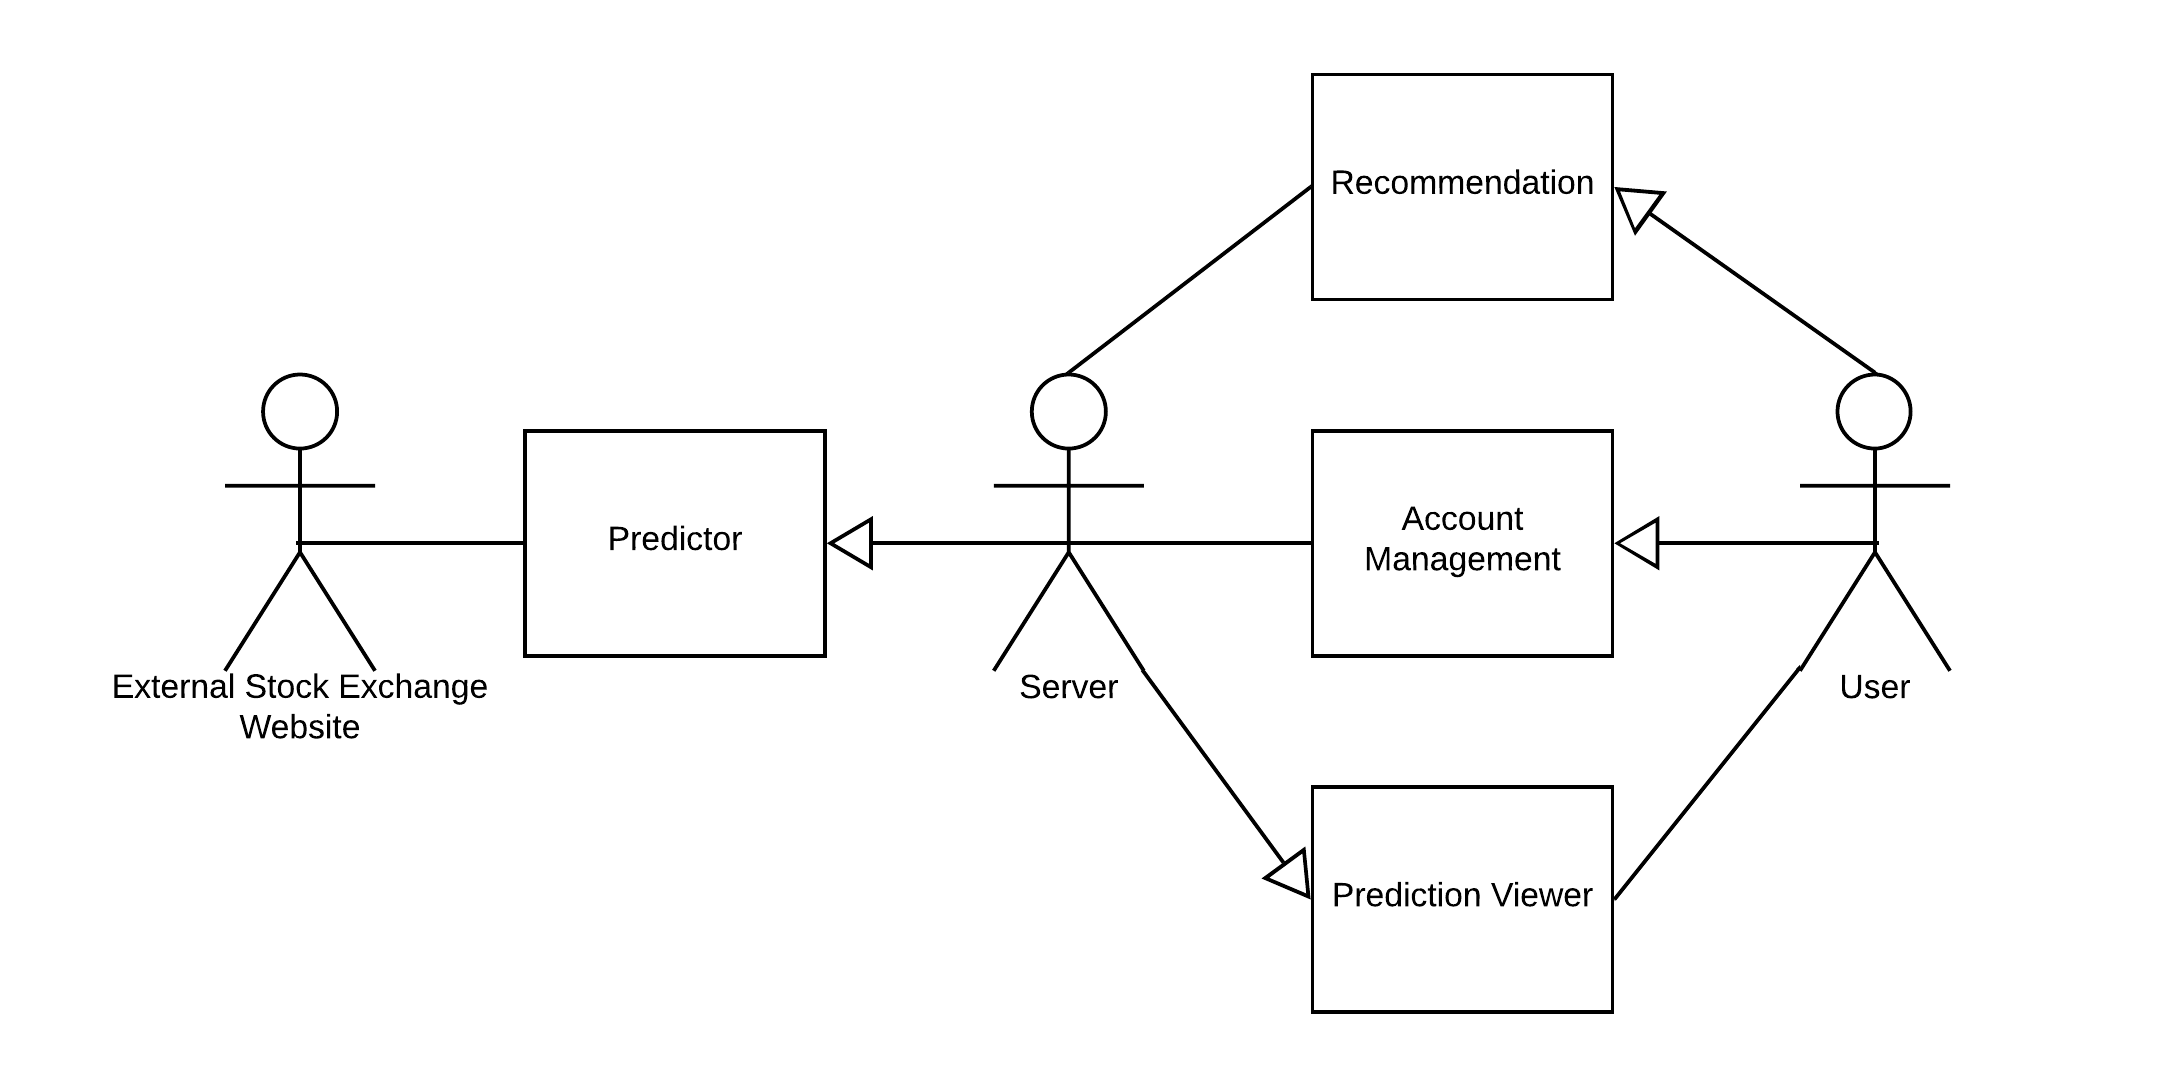
\includegraphics[width=.9\textwidth]{Images/System_Overview.png}
        \caption{System Overview}
    \end{figure}



\newpage
\section{Use Case Diagram}

    In figure \ref{fig:USD_Predictor}, use case diagram of Predictor subsystem is shown. This subsystem handles the collection of data from external stock exchange websites. So the server initiates collection and prediction which is finally saved in database.

    \begin{figure}[!h]
        \centering
        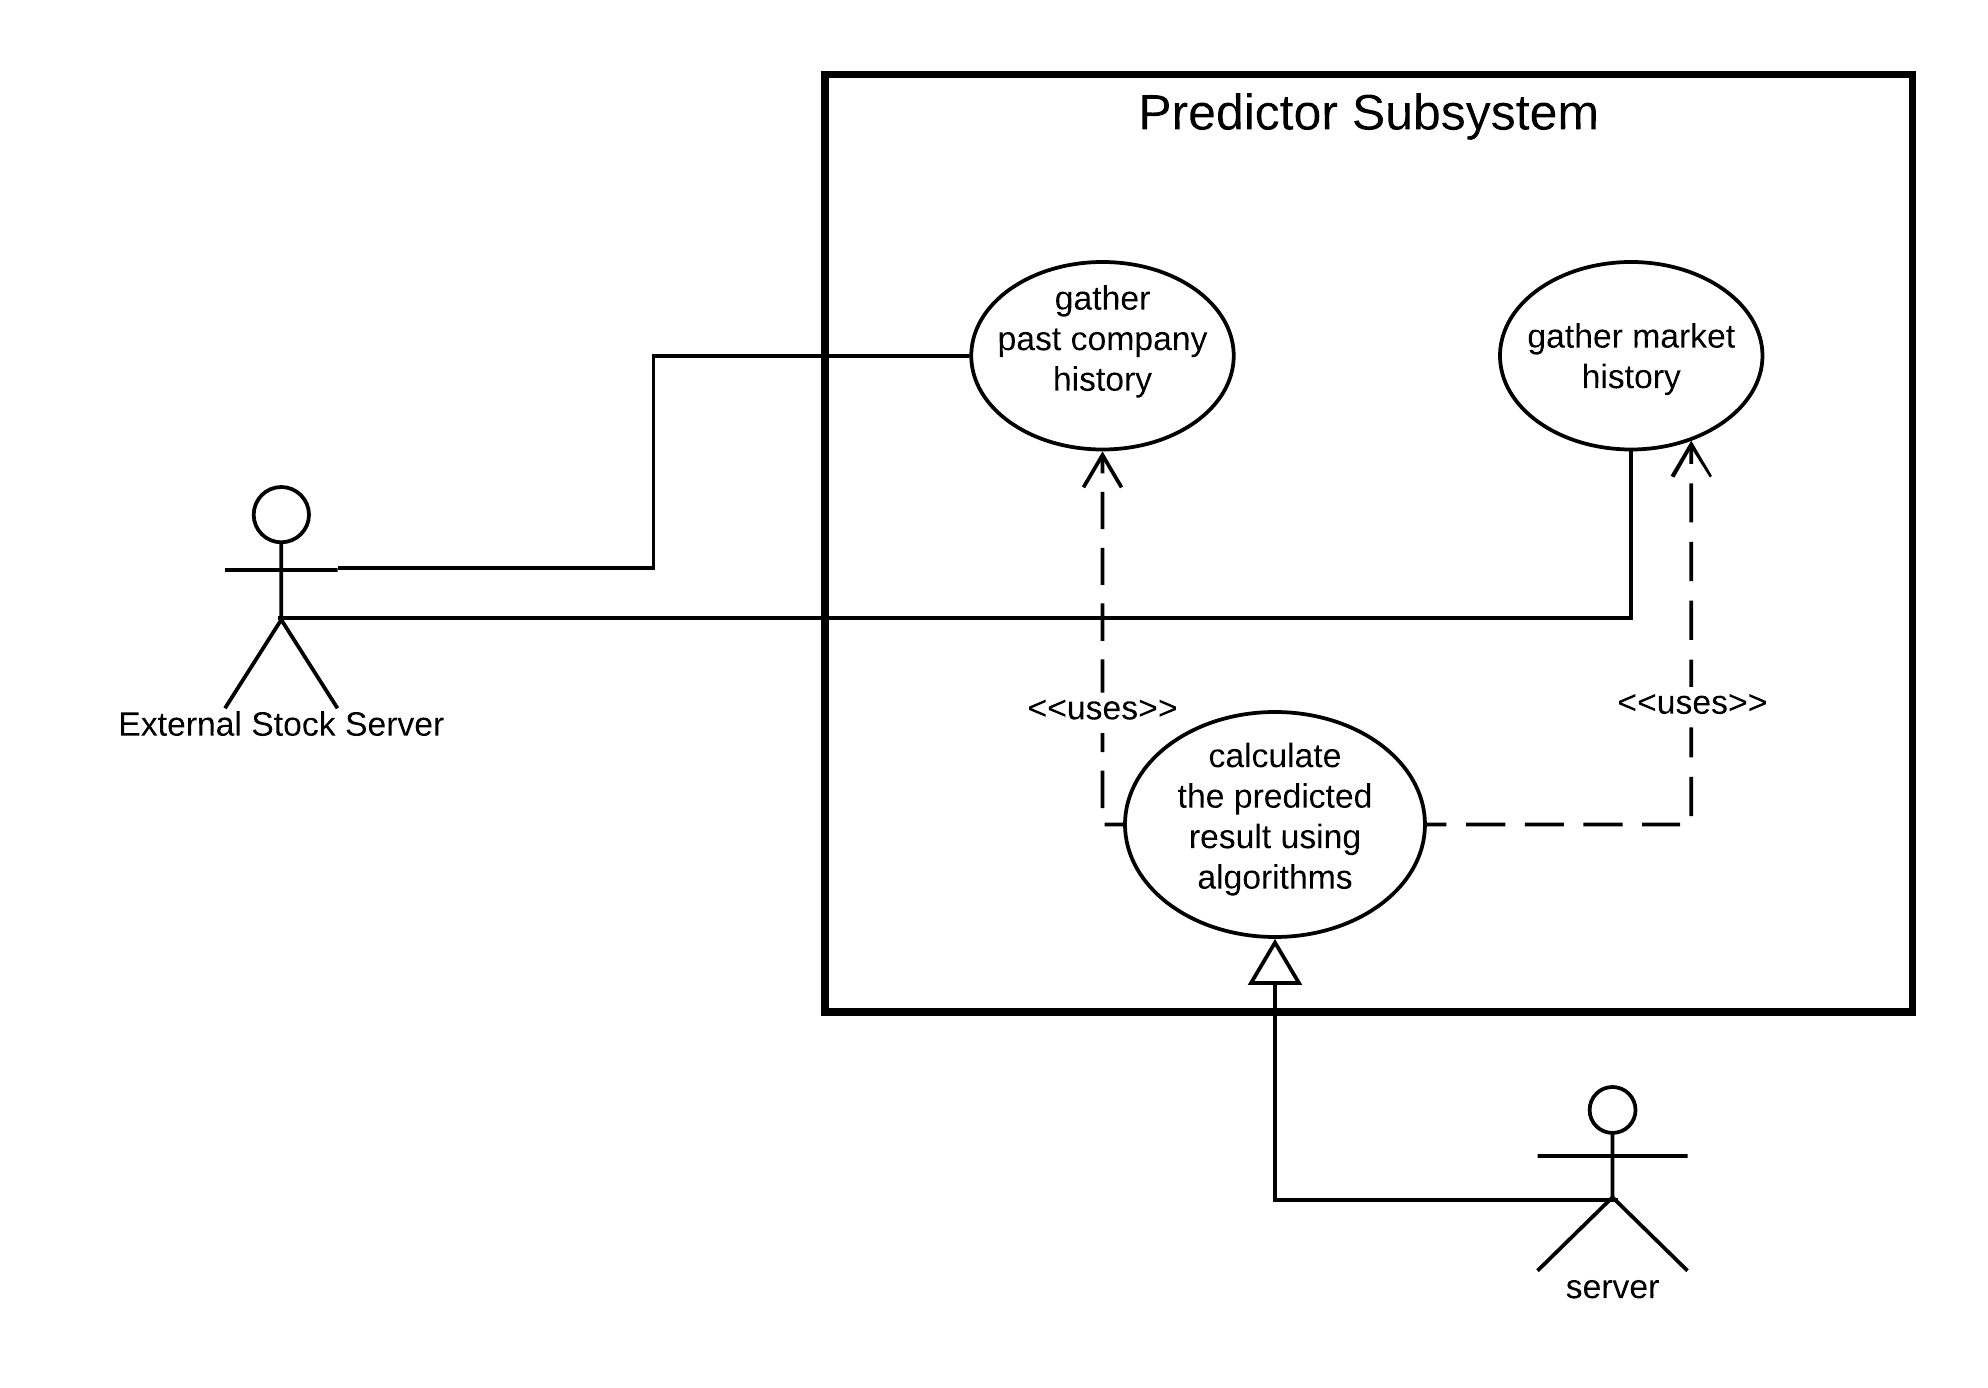
\includegraphics[width=.9\textwidth]{Images/USD_Predictor.png}
        \caption{Use Case Diagram : Predictor Subsystem}
        \label{fig:USD_Predictor}
    \end{figure}
    
    In figure \ref{fig:USD_Viewer}, use case diagram of Prediction Viewer subsystem is shown. In this use case, server initiates GUI and shows list of companies. The user can either search for a company or Select a company for detailed view.

    \begin{figure}[!h]
        \centering
        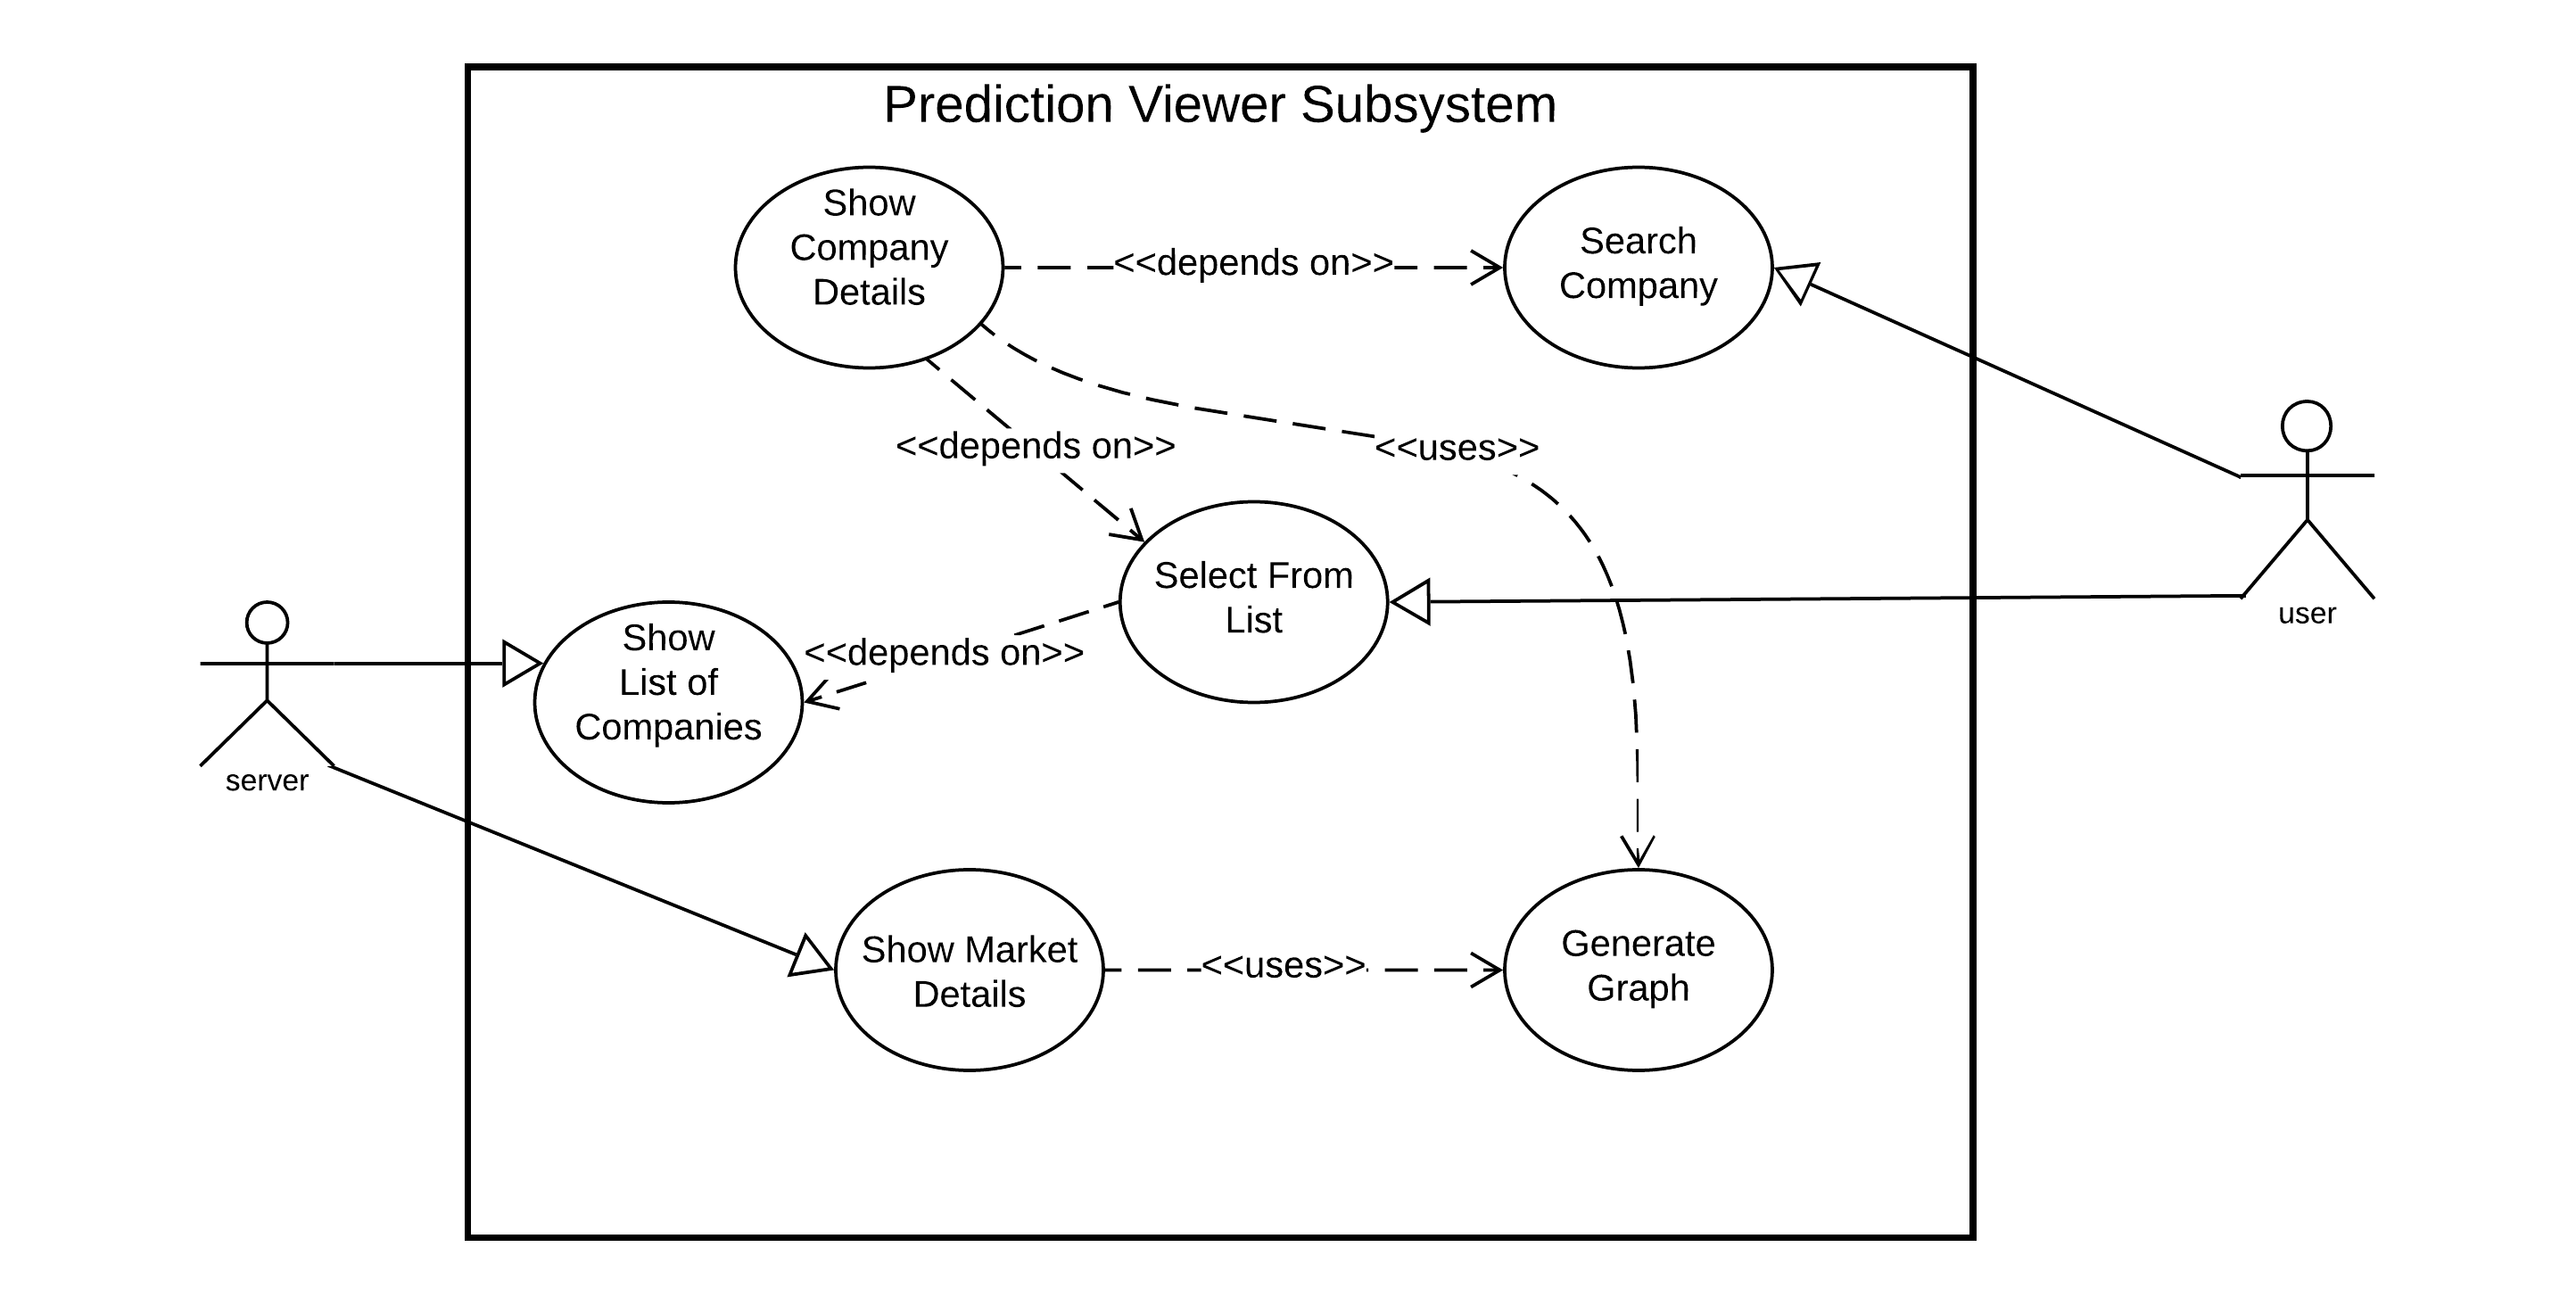
\includegraphics[width=.9\textwidth]{Images/USD_Viewer.png}
        \caption{Use Case Diagram : Prediction Viewer Subsystem}
        \label{fig:USD_Viewer}
    \end{figure}


\newpage
\section{Entity Relationship Diagram}
    \begin{figure}[!h]
        \centering
        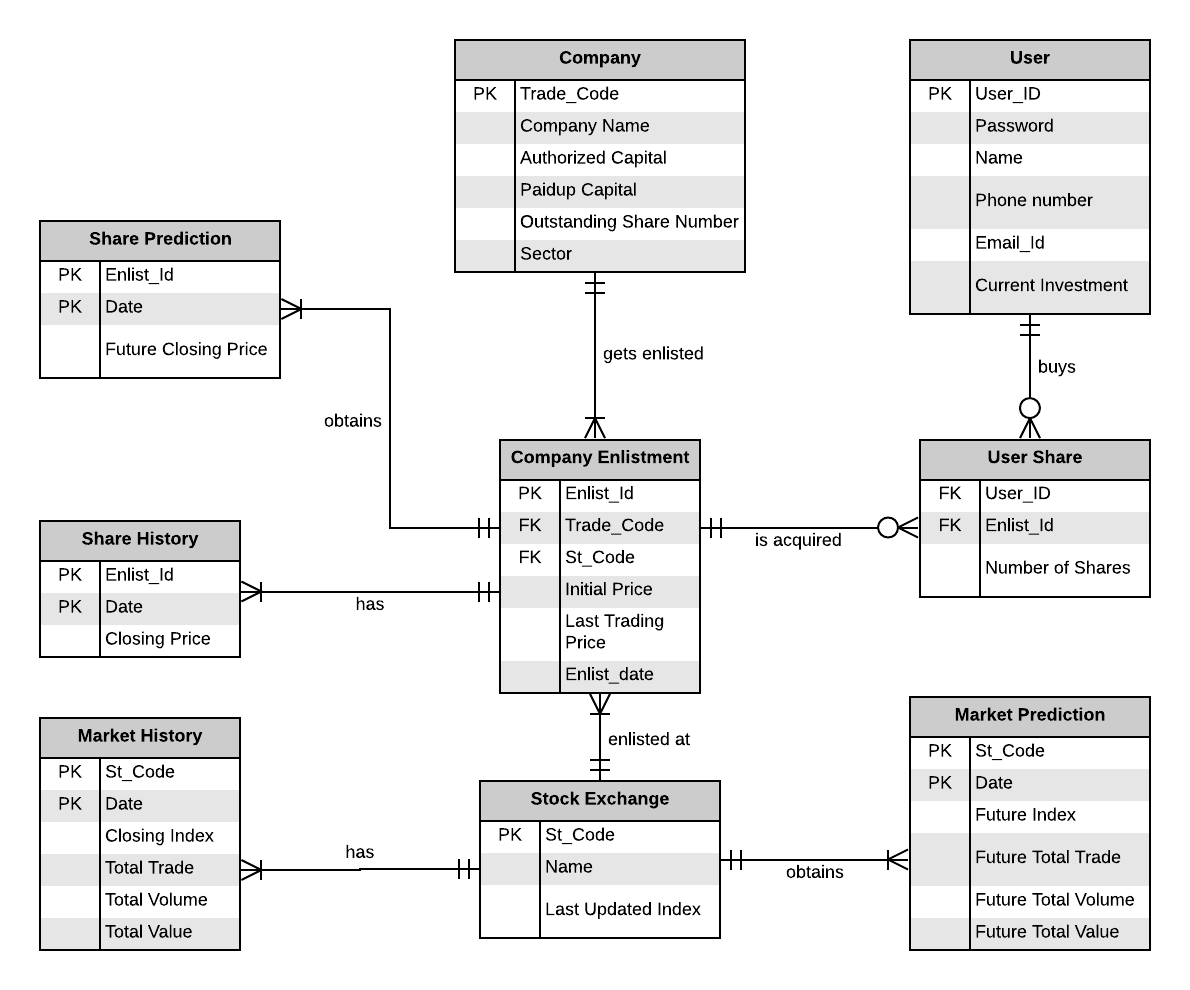
\includegraphics[width=.9\textwidth]{Images/ERD.png}
        \caption{Entity Relationship Diagram}
    \end{figure}
    
    \label{section:ERD}



\newpage
\section{Class Diagram}
    
    \begin{figure}[!h]
        \centering
        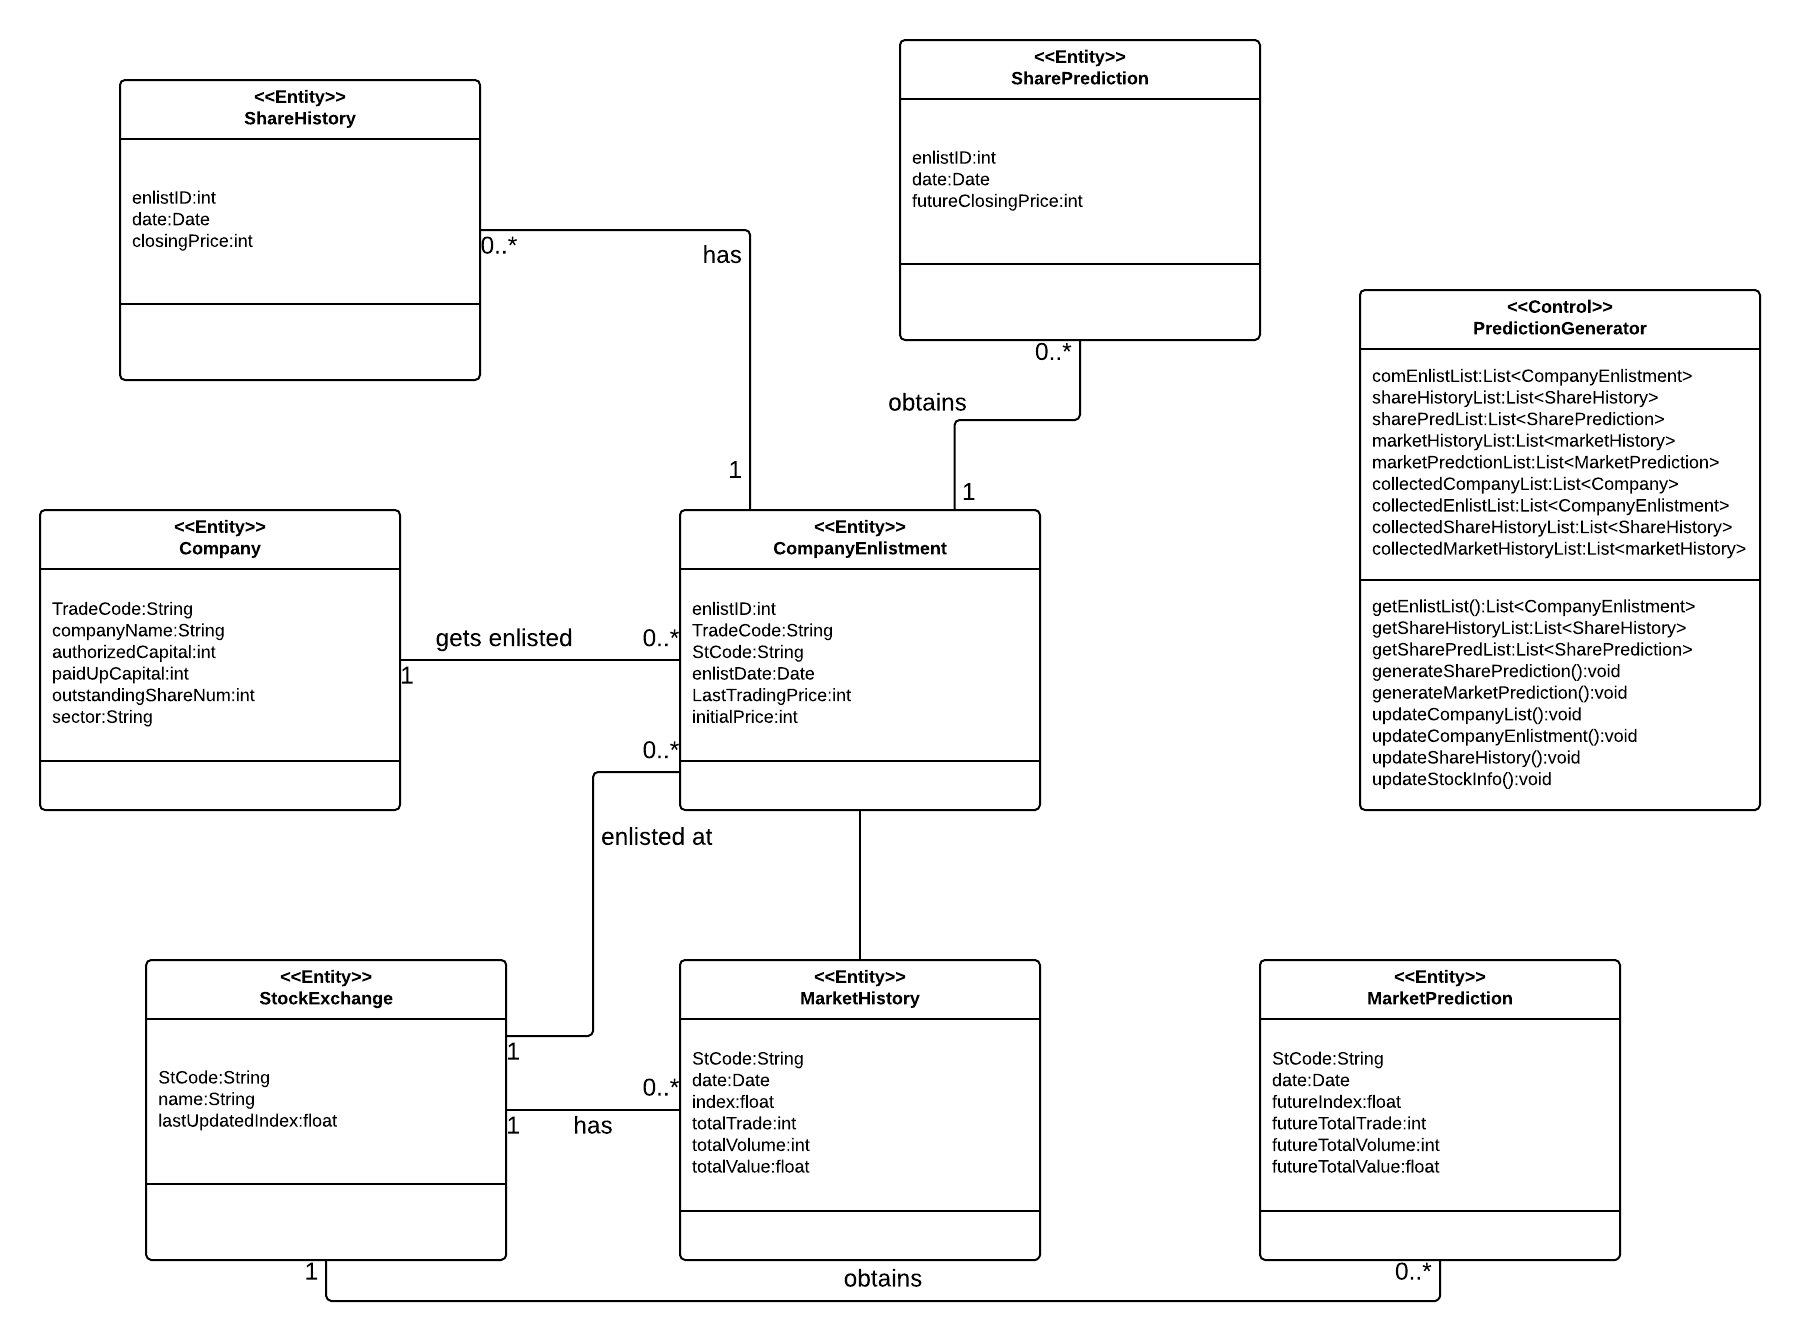
\includegraphics[width=.9\textwidth]{Images/ClassDiagram_Predictor.png}
        \caption{Class Diagram : Predictor Subsystem}
    \end{figure}

    \begin{figure}[!h]
        \centering
        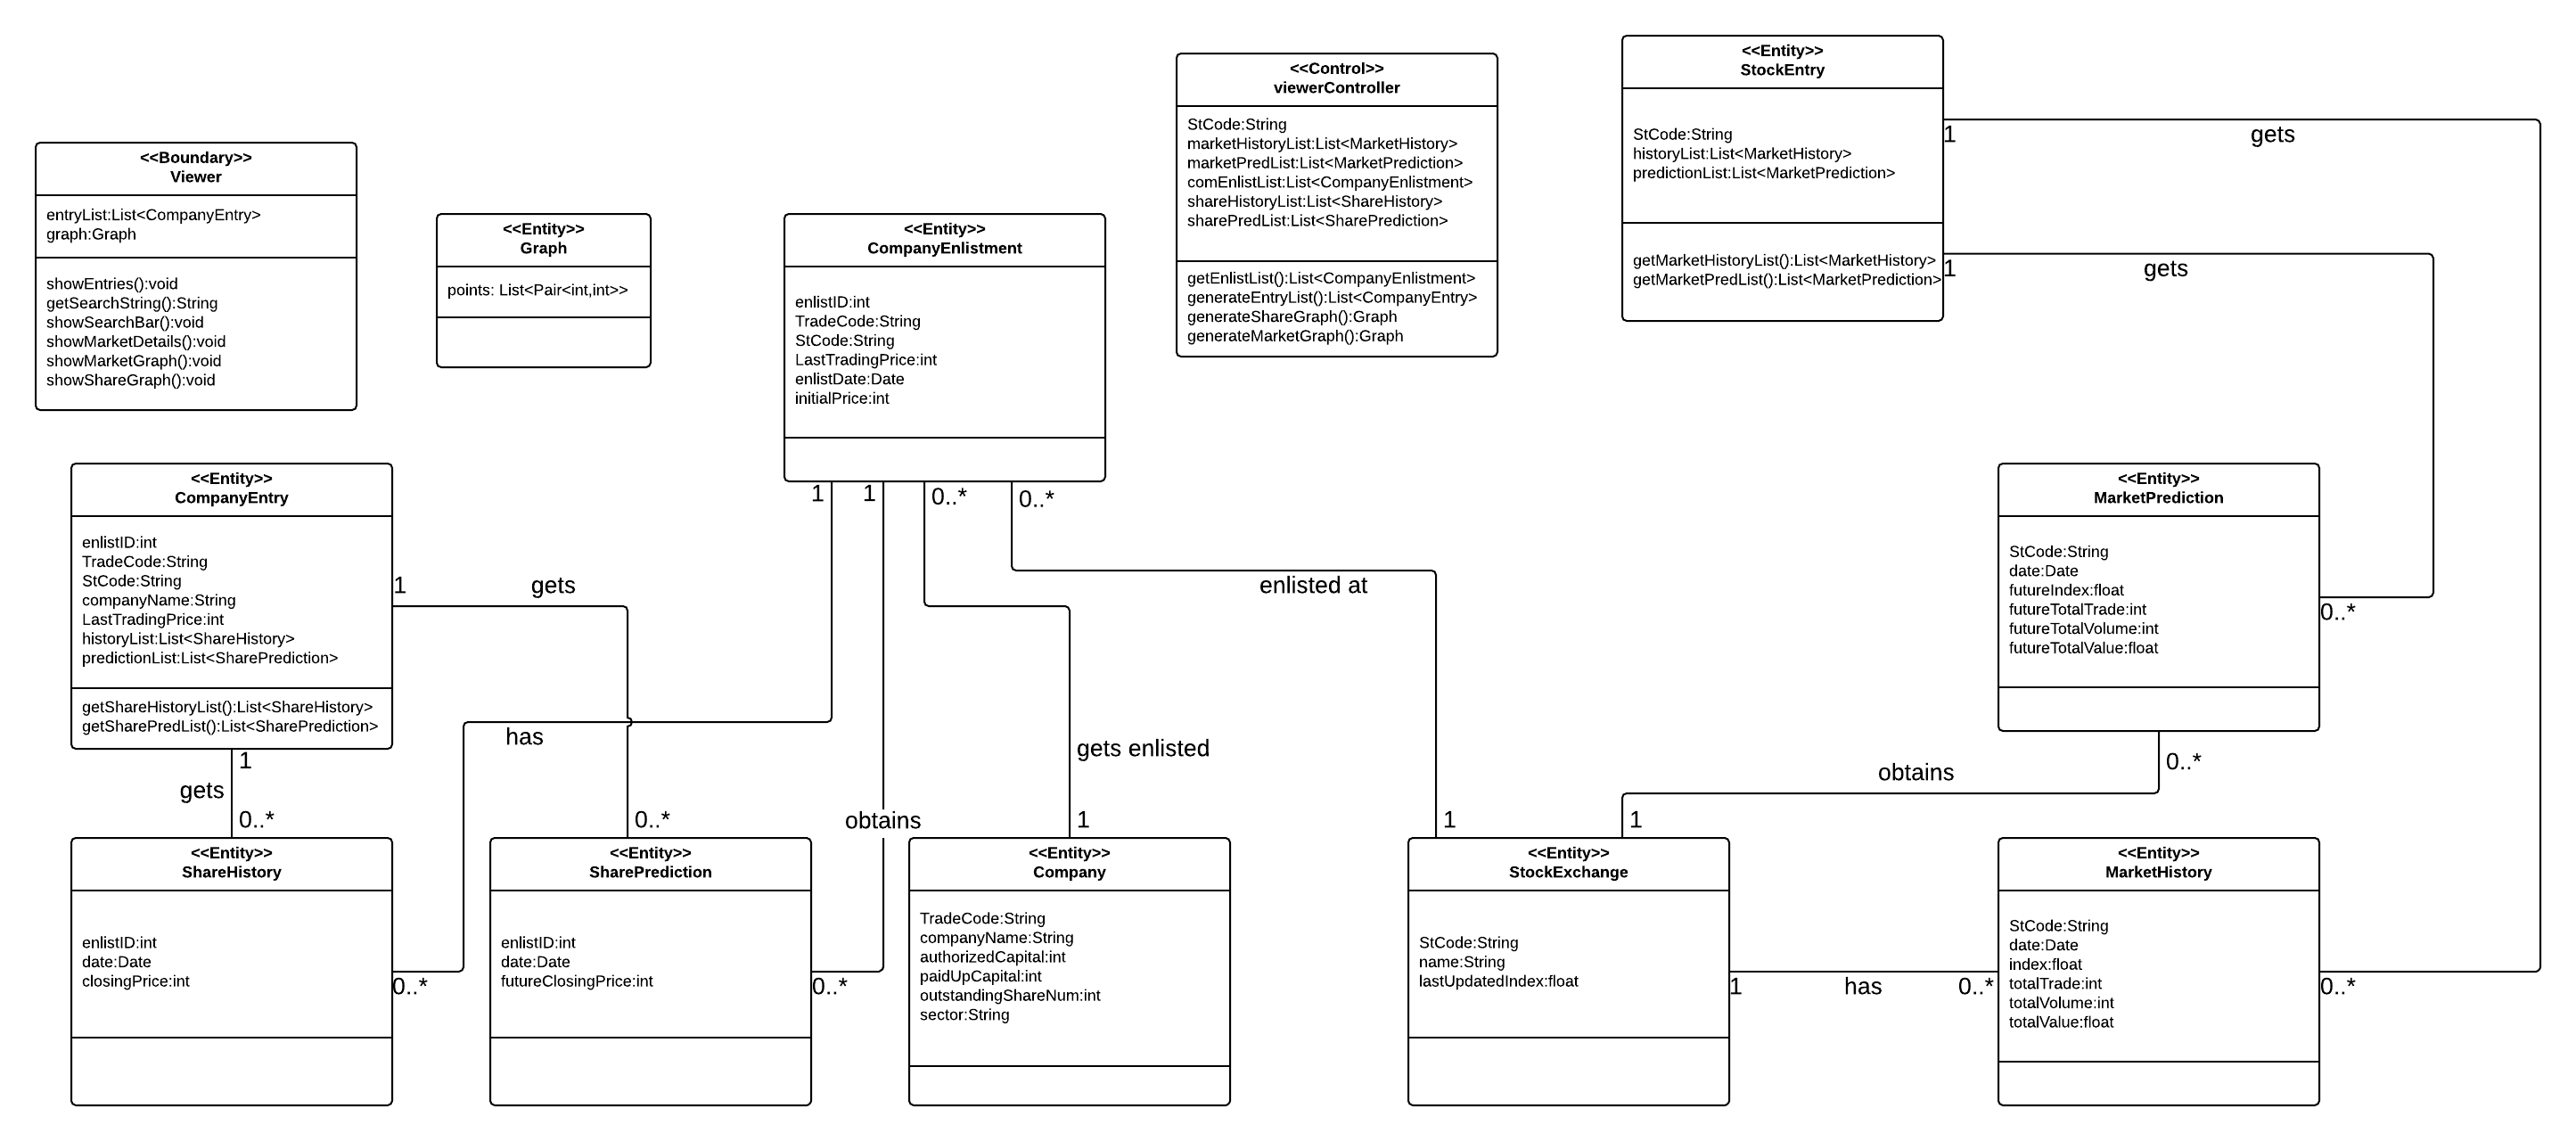
\includegraphics[width=.9\textwidth]{Images/ClassDiagram_Viewer.png}
        \caption{Class Diagram : Prediction Viewer Subsystem}
    \end{figure}



\newpage
\section{Sequence Diagram}

    \begin{figure}[!h]
        \centering
        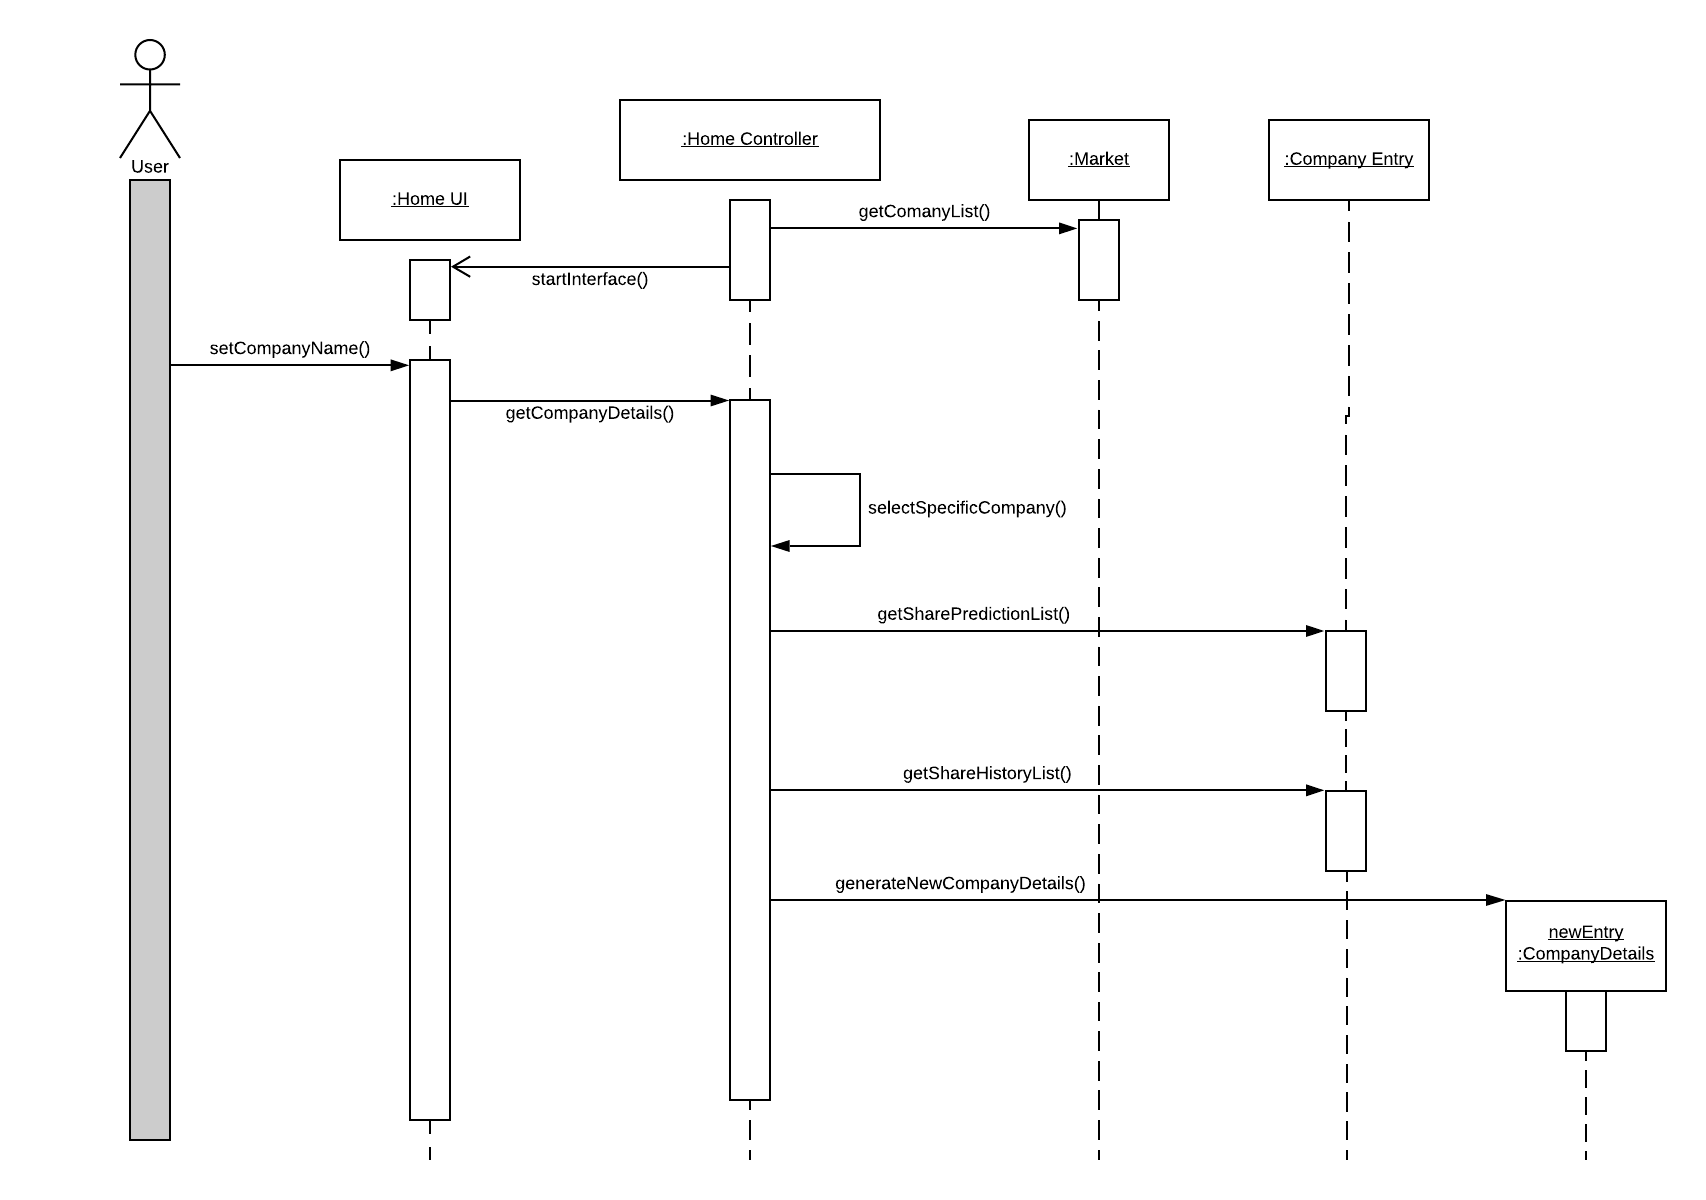
\includegraphics[width=.9\textwidth]{Images/SD_Search.png}
        \caption{Sequence Diagram : Search}
    \end{figure}

    \begin{figure}[!h]
        \centering
        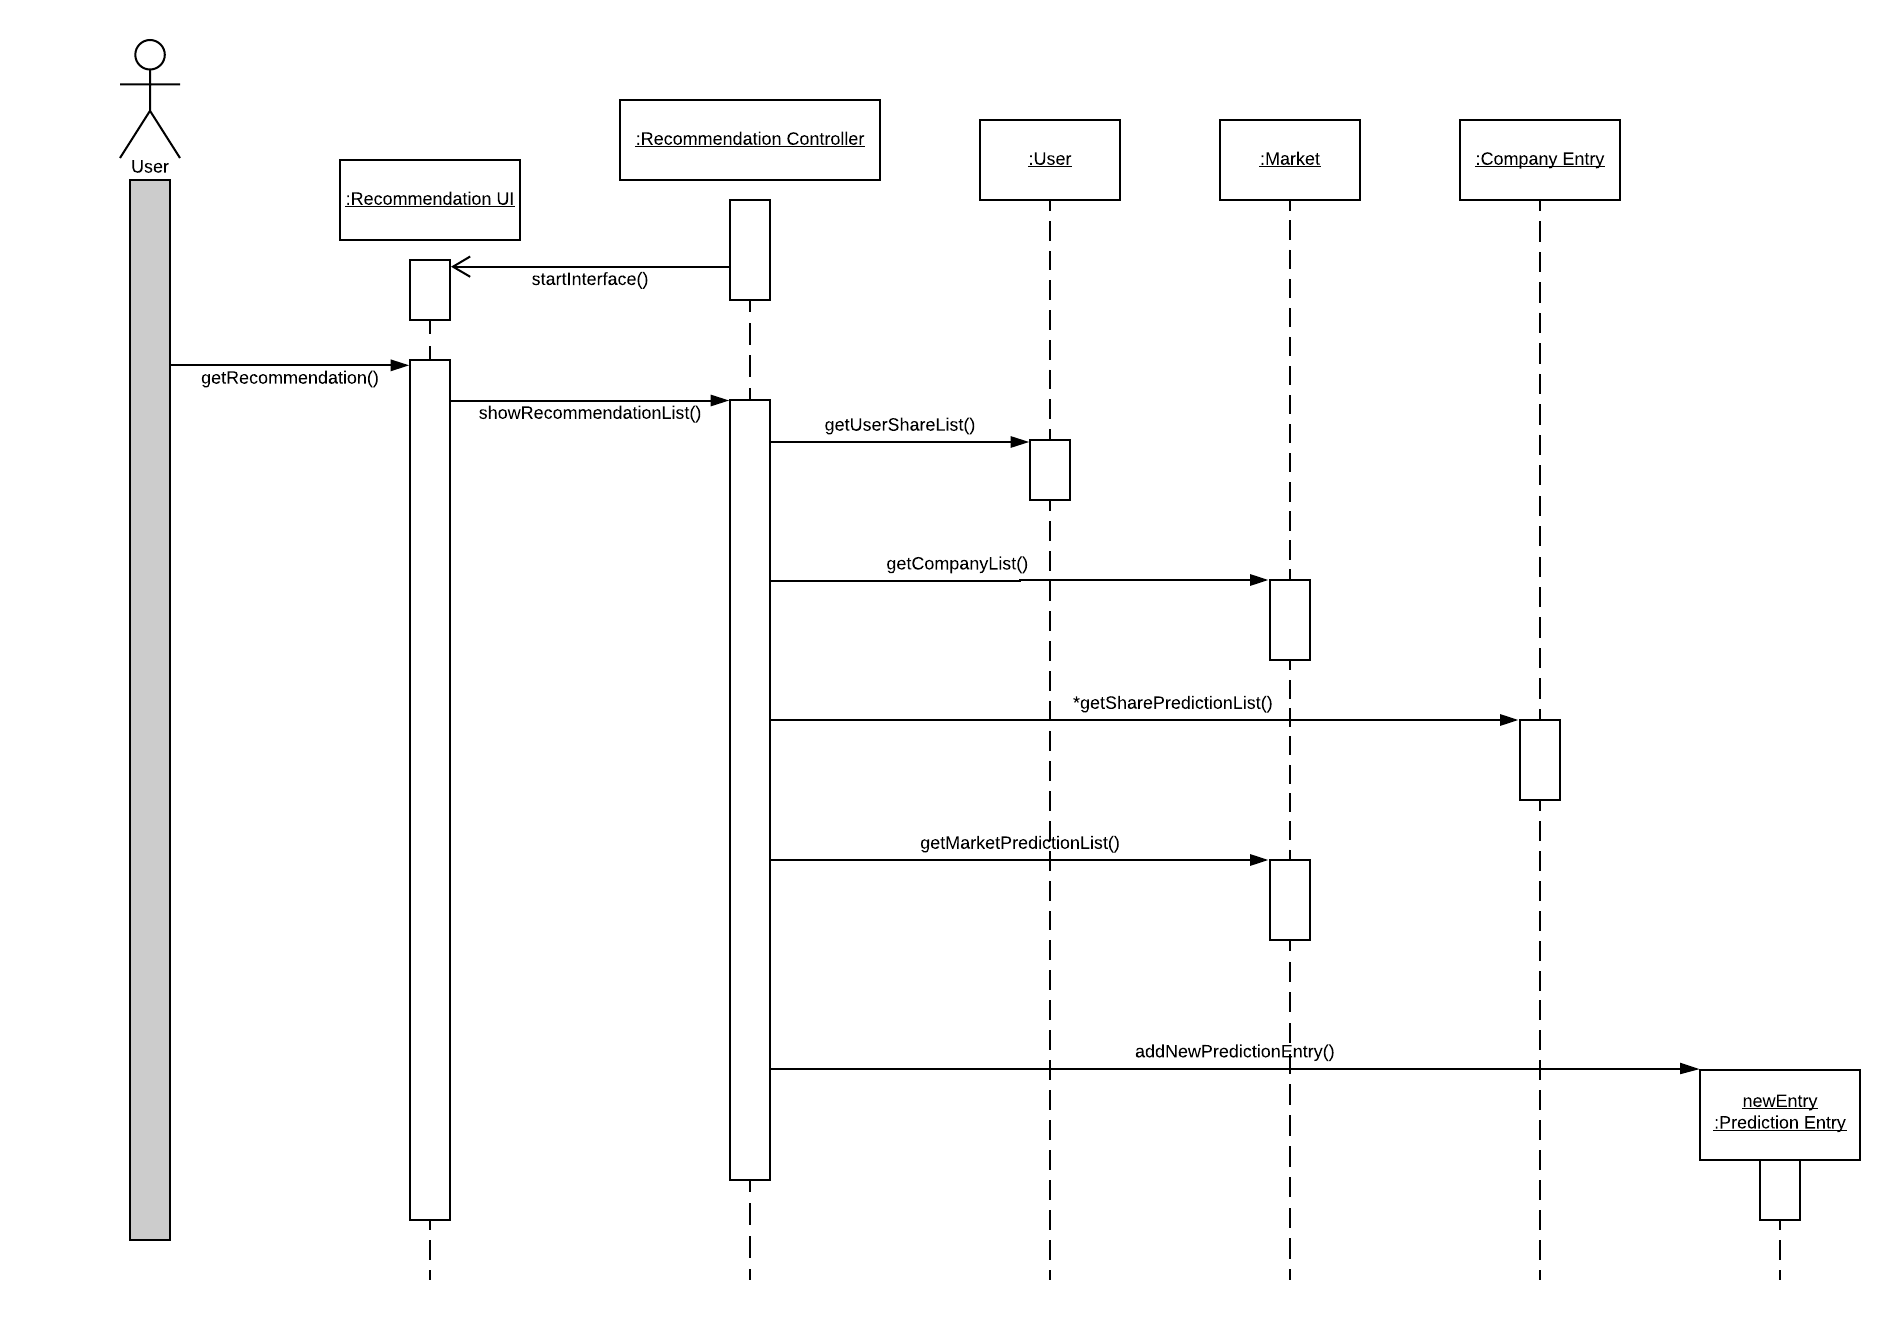
\includegraphics[width=.9\textwidth]{Images/SD_Recommendation.png}
        \caption{Sequence Diagram : Recommendation}
    \end{figure}


\newpage
\section{Data Flow Diagram}
    
    In figure \ref{fig:DFD_Predictor}, physical DFD of predictor subsystem is shown. The business activities of this DFD are: crawl data from stock exchange website, calculate stock prediction and calculate market prediction.
    
    \begin{figure}[!h]
        \centering
        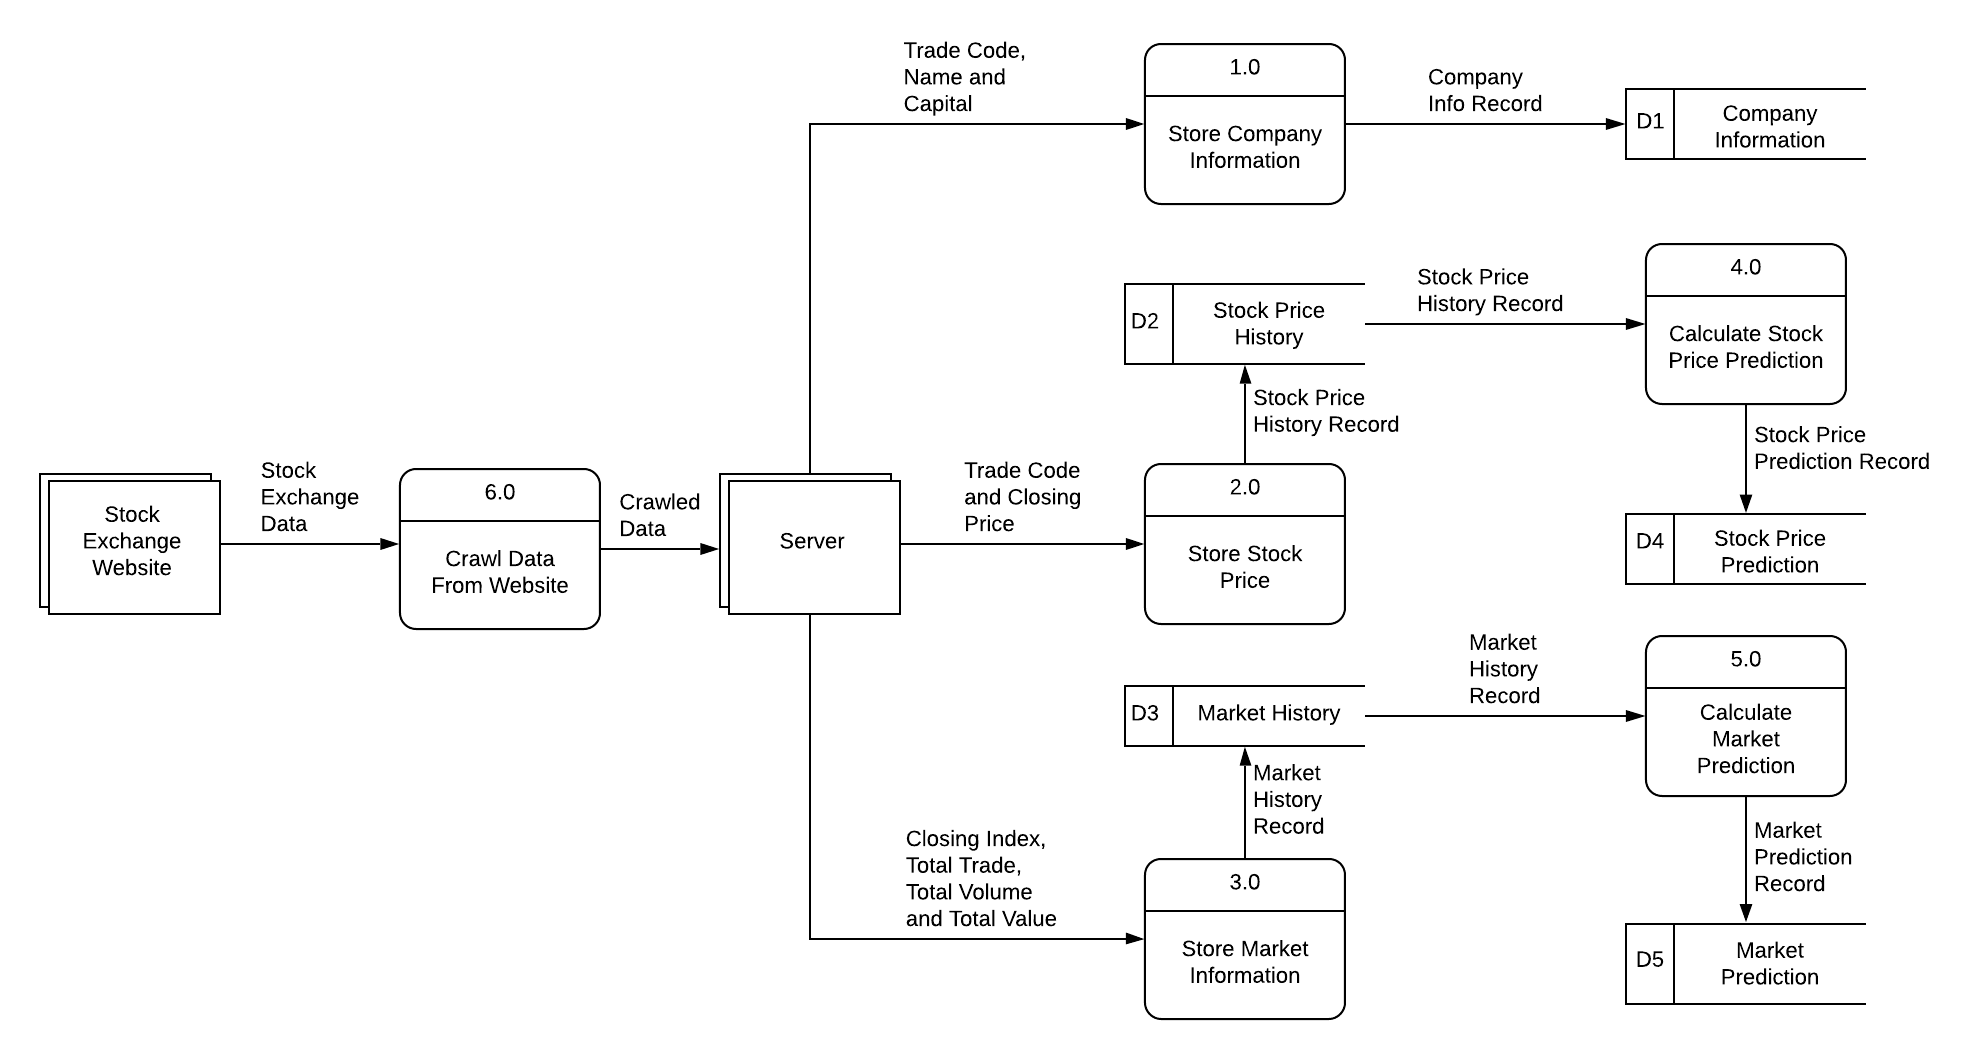
\includegraphics[width=.9\textwidth]{Images/DFD_Predictor.png}
        \caption{Data Flow Diagram : Predictor Subsystem}
        \label{fig:DFD_Predictor}
    \end{figure}
    
    \newpage
    In figure \ref{fig:DFD_Viewer}, physical DFD of Prediction Viewer subsystem is shown. The business activities of this DFD are: generate stock price graph, generate market index graph, search company details, generate company details.
    
    
    \begin{figure}[!h]
        \centering
        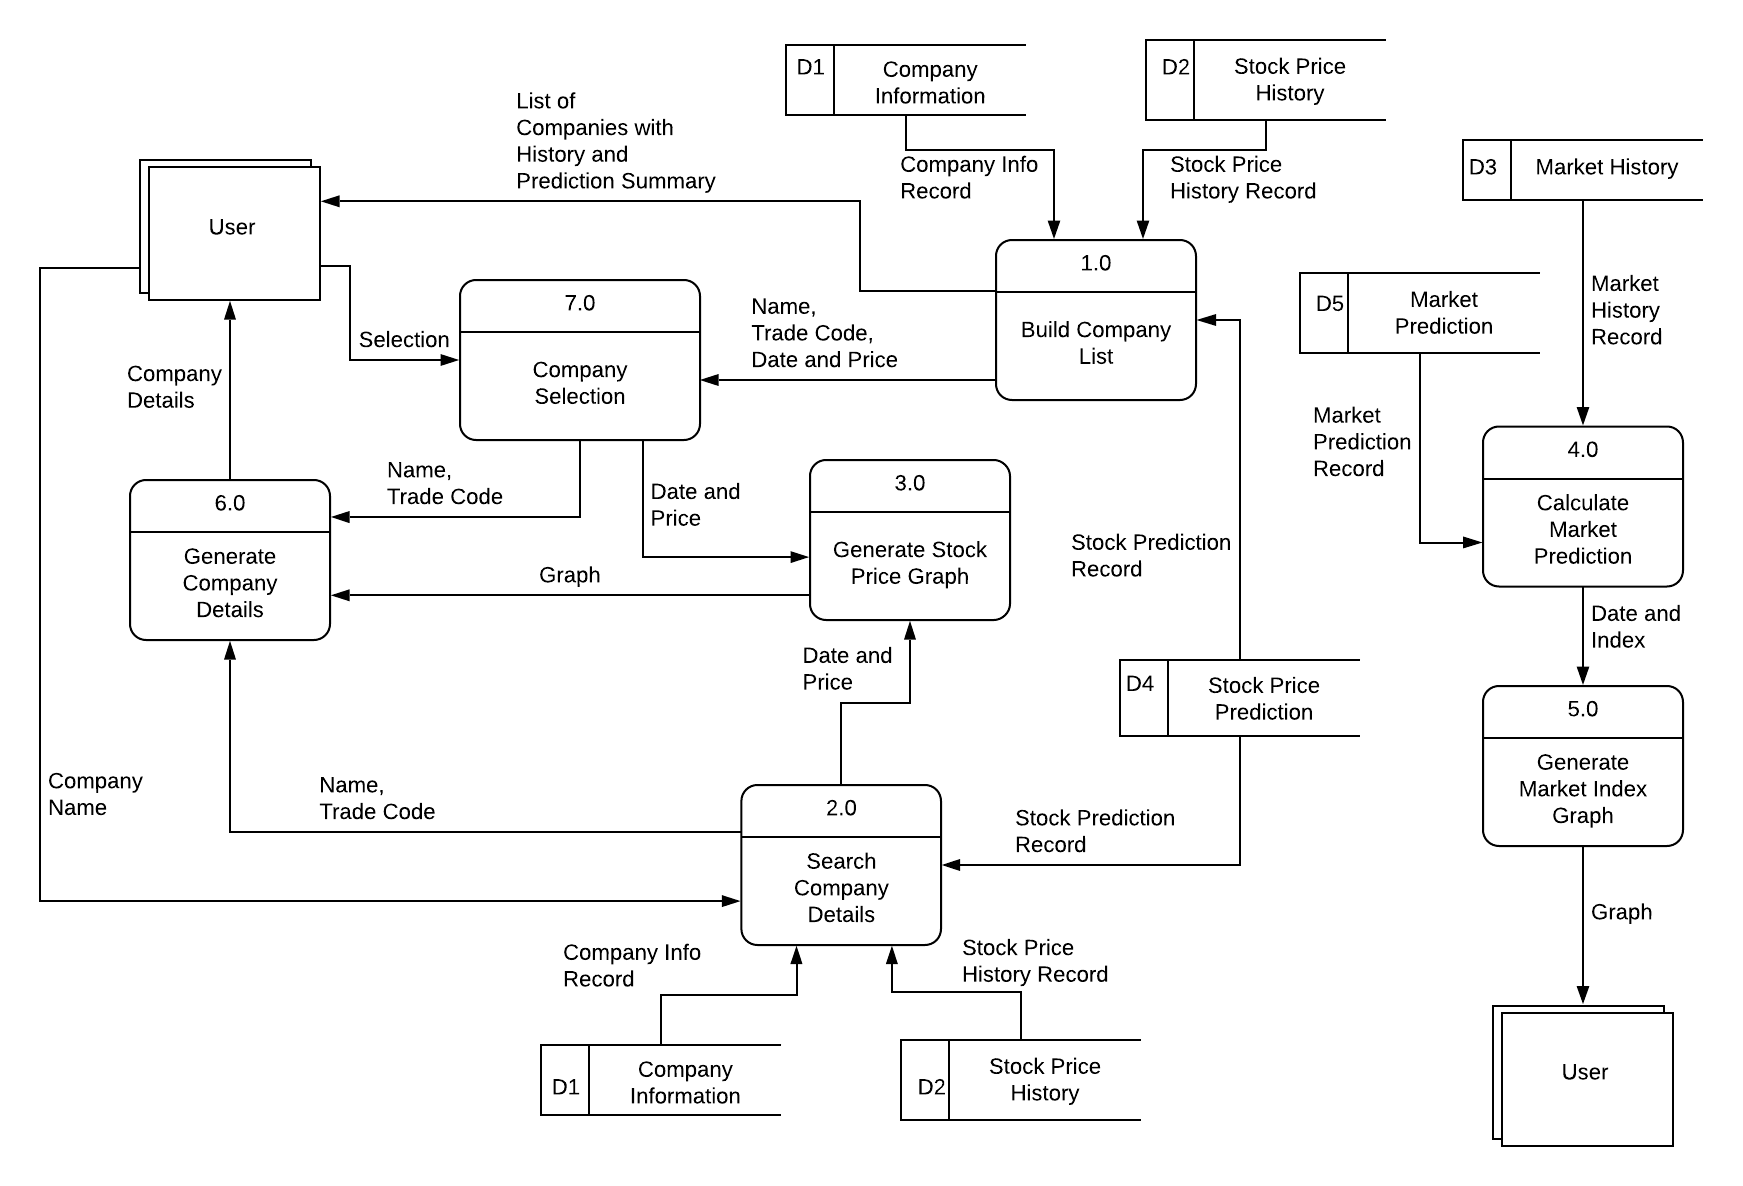
\includegraphics[width=.9\textwidth]{Images/DFD_PredictionViewer.png}
        \caption{Data Flow Diagram : Prediction Viewer Subsystem}
        \label{fig:DFD_Viewer}
    \end{figure}

    


\newpage
\section{Gantt Chart}
    
    \begin{table}[!h]
        \centering
        \begin{tabular}{|c|c|c|} \hline
            Activity & Detailed Activity & Days Required \\ \hline
            
            \multirow{4}{*}{Input/Output Design} & Input Design & 2 \\ 
                & Data validation design & 3 \\ 
                & Data validation design & 3 \\ 
                & Output Design & 2 \\ \hline
                
           \multirow{3}{*}{Prototyping} & Prototype Design & 1 \\ 
                & Prototype Development & 3 \\ 
                & Prototype Evaluation & 2 \\ \hline     
                
            \multirow{7}{*}{Implementation} & Input Design & 2 \\ 
                & Database development & 5 \\ 
                & Stock site crawler development & 7 \\ 
                & Predictor implementation & 10 \\ 
                & Signup/login development & 5 \\ 
                & GUI Implementation & 5 \\ 
                & Investment Recommendar implementation & 10 \\ \hline    
             
             \multirow{3}{*}{Integration} & Unit integration & 7 \\ 
                & Integration testing & 5 \\ \hline   
            
            \multirow{3}{*}{Beta Testing} & Beta version deployment & 1 \\ 
                & User feedback & 10 \\ 
                & Software Update & 7 \\ \hline
            
            Software Release & Software Release & 3 \\ \hline
 
                
        \end{tabular}
        \caption{Activities}
            
    \end{table}

    
    \begin{figure}[!h]
        \centering
        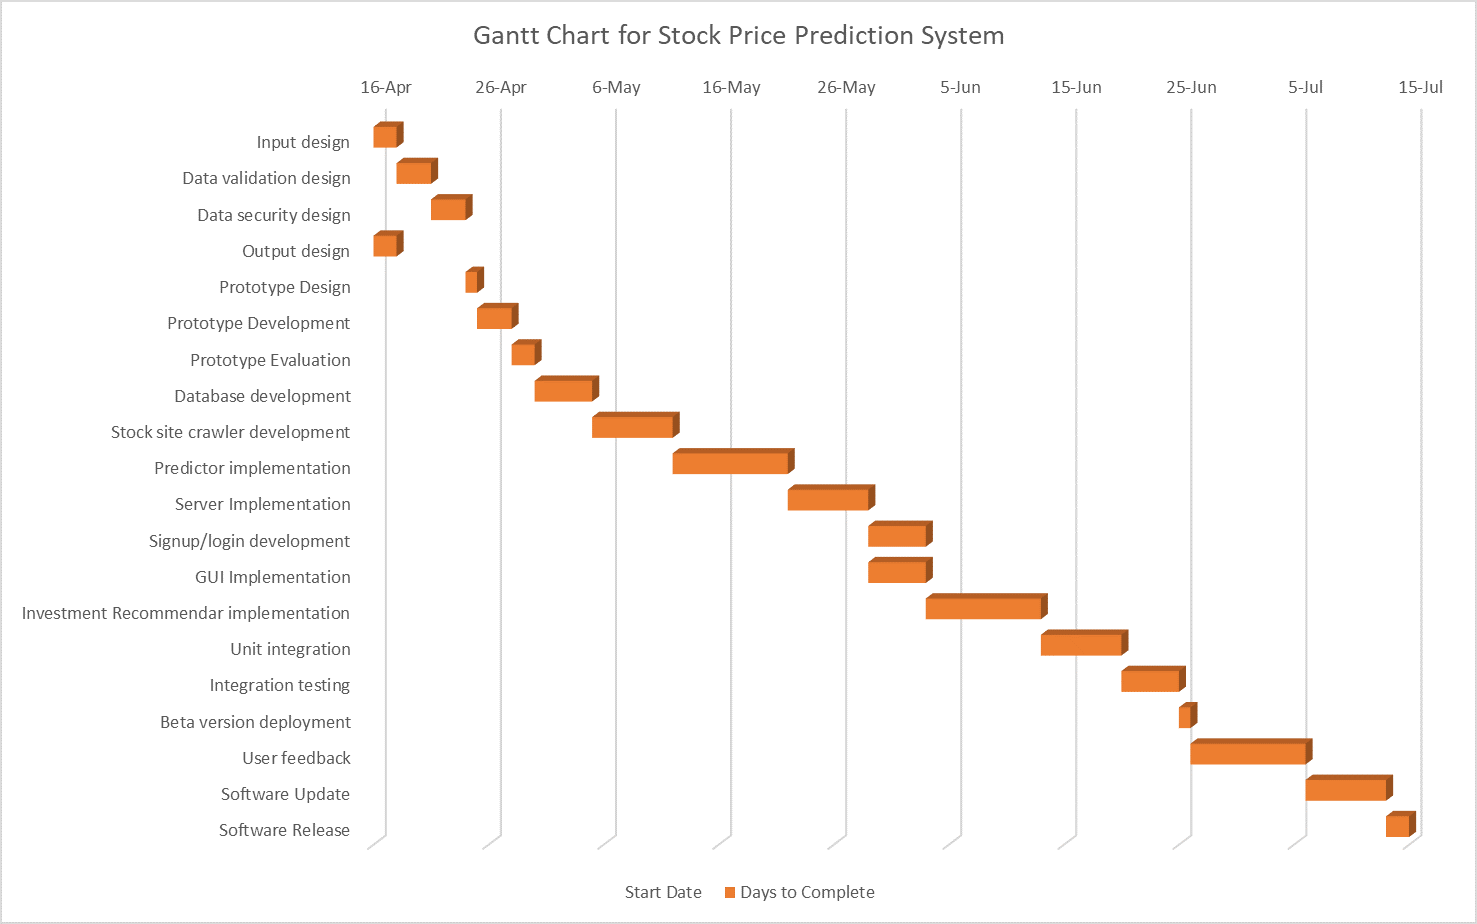
\includegraphics[width=.9\textwidth]{Images/GanttChart.png}
        \caption{Gantt Chart}
    \end{figure}
    

\newpage
\section{Implementation Examples}
    We have implemented the server and the prediction viewer subsystem. To test these, we have also created the database in MySQL according to ERD shown in section \ref{section:ERD} and imported dummy data. The server is taking requests from viewer and responds accordingly with data from database.  \\
    
    In figure \ref{fig:UI}, starting UI is shown. A summary of stock market is shown graphically. The user can also search by trade code in the search bar. Search results example can be seen in figure \ref{fig:Search}. Selecting a company brings company details window. It includes graphical representation of history and prediction of the particular company. This window is shown in figure \ref{fig:complanyDetails}.
    
    \begin{figure}[!h]
        \centering
        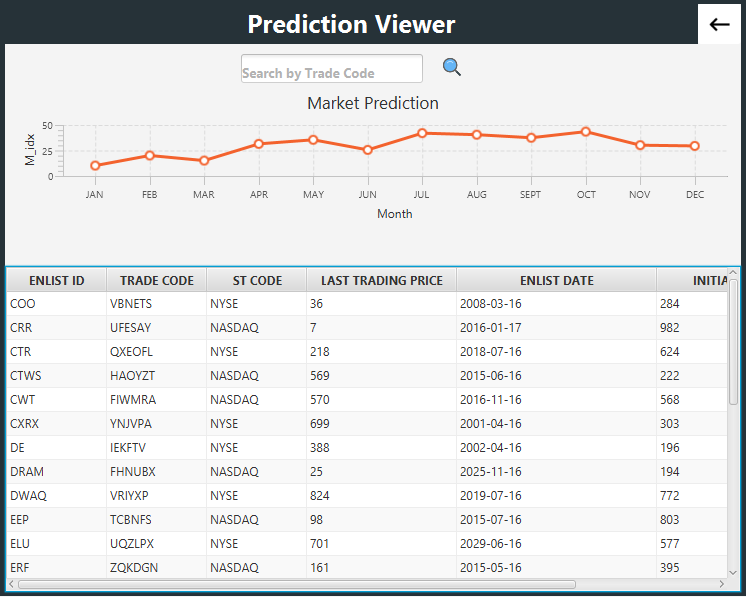
\includegraphics[width=.9\textwidth]{Images/SS1_All.PNG}
        \caption{Example : Starting UI}
        \label{fig:UI}
    \end{figure}
    
    \begin{figure}[!h]
        \centering
        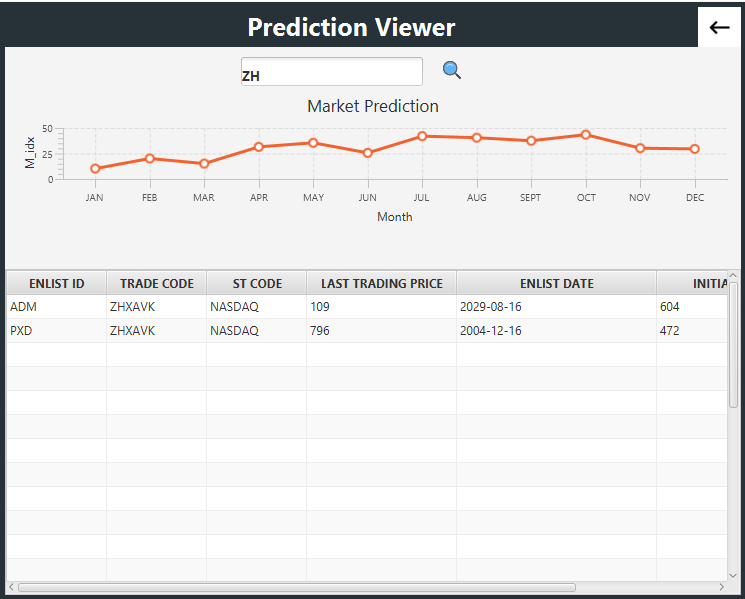
\includegraphics[width=.9\textwidth]{Images/SS2_Search.PNG}
        \caption{Example : Search}
        \label{fig:Search}
    \end{figure}
    
    \begin{figure}[!h]
        \centering
        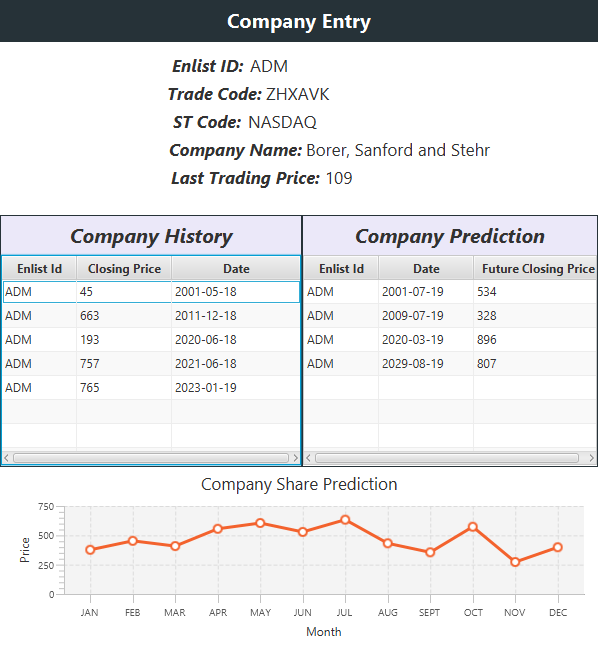
\includegraphics[width=.9\textwidth]{Images/SS3_Details.PNG}
        \caption{Example : Company Details}
        \label{fig:complanyDetails}
    \end{figure}
    


\section{Conclusion}
We have included the use case diagrams for 2 subsystems, ERD of the database, Class diagram and DFD for 2 subsystems and sequence diagram for 2 use cases in this report. Also, we have included the Gantt chart of the project which will start in mid-April in this report.

Stock price prediction system can have a huge impact in the day-to-day life of the stock investors if it is implemented intelligently. So, we are following the software design and development procedures to the point for implementing this software which is the main objective of this course. 



\end{document}